\section{Experiments}
\subsection{Evaluation metrics}
In order to evalute the performance of the different algorithms, three different metrics were used. For each of these methods we hold on to the closed world assumption that if a link is not present within the given data set, it should not be a link. 

\subsubsection{Precision and recall}
Precision and recall can be calculated when the complete system pipeline is used. Precision reflects the fraction of relevant documents from all proposed documents and can thus be calculated as follows:

\begin{align*}
  \textrm{precision} = \frac{|\;\textrm{relevant\;documents} \cap \textrm{retrieved\;documents}\;|}{|\textrm{retrieved\;documents}\;|}
\end{align*}

Recall represents the fraction of relevant documents of all originally linked documents and can be calculated as follows:

\begin{align}
  \nonumber \textrm{recall} = \frac{|\;\textrm{relevant\;documents} \cap \textrm{retrieved\;documents}\;|}{|\;\textrm{relevant\;documents}\;|}
\end{align}
The precision and recall can be unraveled into precesion and recall per document type to give more insight into the performance of the algorithms with regards to different document types. 

\subsubsection{K-links}
The k-links metric is used to evaluate the algorithms, without being influenced by the threshold for the number of proposed links. For a document with a given number of correct links, it proposes the same amount of links that the document is known to have. This evaluation metric thus makes the assumption that the algorithm knows in advance how many links should be returned. By doing so, the recall and precision are equivalent since the number of relevant and retrieved document is the same. It prevents the precision of being too optimistic, which would be the case if the fixed number would be lower than the actual amount of links. It also prevents the recall for being too optimistic in the cases that the actual amount of links is lower than the fixed number of proposed links. 

The disadvantage of the k-links metric is of course that it does not take into account the certainty the algorithm has due to the distances. For example, it could be that the distance of the first two ranked documents is very small, but the distance of the third is very large. If the original document has 10 links, the system is forced to additionally return the nine documents, even though these are likely to be wrong because they have a relatively big distance. 

\begin{table}
\begin{tabular}{| l | l | l | l | l | l | l | l |}
\hline
 & Inf. &  Question &  Good Pr.& Project & Person &  Event & {\bf Average} \\
\hline
Textvectorizer & 20.22 & 37.99 & 21.53 & 20.16 & 6.15 & 16.07 & {\bf 18.32}\\
Weighted text vectorizer & 23.38 & 38.78 & 21.53 & 16.23 & 7.44 & 16.07 & {\bf 19.58} \\ 
Simple tag similarity & 28.97 & 24.85 & 53.47 & 32.62 & 17.44 & 36.61 & {\bf 26.26} \\
Tag smoothing & 25.79 & 28.36 & 53.47 & 23.97 & 13.59 & 36.61 & {\bf 23.76}\\
Glossaries of tags & 20.68 & 23.80 & 30.56 & 27.06 & 10.51 & 55.36 & {\bf 20.03}\\
\hline
\end{tabular}
\caption{Percentage of links from one type (row) to another (column) for the real links in the document base}
\label{klink}
\end{table}

\subsection{Text-based descriptors}
Table \ref{klink} shows the k-link values of the text-based descriptions: the textvectorizer and the weighted-text vectorizer. On average, 18.32\% and 19.58\% percent of the number of proposed links respectively are correct. The weighted text vectorizer performs a bit better, which is mainly due to an improvement in performance on information, questions and persons. SOME QUALITATIVE EXAMPLES ARE STILL NEEDED HERE. Though performance on Persons has improved by adding the weights, both textvectorizers have a low precision with regards to proposing links for Persons. This could by explained by the fact that about 76.36\% (not weighted) and 63.64\% (weighted) of the links for Persons are towards other Persons. However, within the Starfish network such links almost never occur (see table \ref{bayes_table3} for the distribution of document types within Starfish).

Overall, both textvectorizers are slow in performance even though the corpus is small. Additionally, the the bag-of-words approach imposes a few limitations on the document linker. Firstly, it performs bad when different languages are used. Figure x shows the differences of vectors of three texts when an English document is combined with an English proposed document and a Dutch proposed document. In the case of two different languages, there are less words that the two documents have in common. If important keywords entail word such as 'clickers' versus 'stemsysteem', there is no way of relating the two documents. Secondly, the current StarFish network consists of mainly textual content. However, in the future this is likely to be extended with images, videos and other non-textual content. These sources should then somehow be converted to text.

\subsection{Tag-based descriptors}

\subsubsection{Simple tag similarity vectorizer}
The performance of the simple tag similarity vectorizer, as shown in table \ref{klink} together with the other tag vectorizers, is about 26\% precision when measuring k-link. The unraveling per document type shows that Question documents and Person documents perform the least. This can be explained by the fact that half of both Questions and Persons have zero tags. Obviously, the simple tag vectorizer cannot deal with such documents. In fact, almost all other Questions have only one tag. Since the simple tag vectorizer compares vectors, it wil prefer documents that also have only that particular tag, which makes it sensitive to attaching Questions to Questions. Something similar seems to happen with Persons, of which 50.91\% of the connections are with other Persons. Apparently, persons with similar expertices are tagged similarly. However, as mentioned with the text vectorizer, in Starfish persons almost never refer to other persons. Moreover, if a document is badly labeled this can also induce problems. For example, take the question 'Is there an English version in Tentamenlade', tagged with 'ToetsenEnToetsgestuurdleren'. The proposed links are visible in table \ref{proposed}, which shows that  the three proposed questions all have the tag 'ToetsEnToetsGestuudLeren'. However, if the question was tagged with the tag 'Tentamenlade', which seems very reasonable given the proposed question, the false negatives would likely be returned correctly by the system. Good practices, events and projects perform better, but these document types only entail 3.2\%, 2.7\% and 5.4\% of the total amount of documents respectively so have less influence on the average precision.

\begin{table}
\begin{lstlisting}
False Positives:
- Wat is het verschil tussen Learning Analytics en TTL (Question)
- Formatieve meerkeuze toetsen om begin kennisniveau te toetsen (Good Practice)
- De toetscyclus (Information)

True Positives:
- Tentamenlade2.5 (Project)

False Negatives:
- Tentamenlade Natuurkunde (Information)
- Hoe kan ik inloggen in Tentamenlade? (Question)
- Hoe kan ik inloggen in Tentamenlade? (Question)
\end{lstlisting}
\caption{Proposed links for the question 'Is there an English version in Tentamenlade?'}
\label{proposed}
\end{table}

\subsubsection{Tag smoothing}
The performance of the simple tag vectorizer, as shown in table \ref{klink}, is quite similar with the results of the tag similarity. It performs worse on the information, but better on questions. EXAMPLE THAT EXPLAINS WHY. It also performs worse on Persons. EXAMPLE THAT EXPLAINS WHY. 

In the current implementation this vectorizer is relatively slow. In practice the similarity matrix can be pre calculated and updated in batches. Due to the transform on the tag similartity matrix, it is very hard to determine which tag occurrences contributed to the document similarity and why some recommendations are made. It does not seem to perform much better than the regular bag of words tag descriptor, in \citeauthor{zhou2011web} the algorithm only starts performing significantly better when it is presented with more tags.

\subsubsection{Glossaries of tags}
To be continued.

\subsection{Bayesian weighting}
\begin{table}
\begin{tabular}{| l | l | l | l | l | l | l | l |}
\hline
 & Inf. &  Question &  Good Pr.& Project & Person &  Event & {\bf Average} \\
\hline
Textvectorizer & 3.68 & 11.23 & 0.00 & 0.00 & 0.51 & 0.00 & {\bf 3.21}\\
Weighted text vectorizer & 3.60 & 11.23 & 0.00 & 0.00 & 0.51 & 0.00 & {\bf 3.19} \\ 
Simple tag similarity & 4.56 & 20.24 & 15.55 & 0 & 0.51 & 25.00 & {\bf 6.70}\\
Tag smoothing & 4.69 & 18.48 & 33.33 & 0.00 & 0.51 & 0.00 & {\bf 6.46}\\
Glossaries of tags & 5.35 & 20.24 & 0.00 & 3.93 & 8.21 & 25.00 & {\bf 9.02}\\
\hline
\end{tabular}
\caption{Percentage correct links per vectorizer per document type after a k-link measurement}
\label{bayes_table1}
\end{table}

Table \ref{bayes_table1} shows the performance of each of the vectorizers (all with cosine distance) while applying the tag and link devaluation using the k-link metric. It shows that the performance of all algorithms drastically decreases when the probabilities are used to re-rank the documents. Table \ref{bayes_table1}  shows the distribution of links in the simple tag similarity vectorizer, with and without the probabilities (all based on k-link measuring). It is clear that the links with probabilties have a sharper distribution: the sparseness of the table shows that many types of links do not even exist. This effect could be caused by overfitting - the data set could be too small to calculate reliable probabilities. The prefered effect of having no Persons link to other Persons was done correctly. However, Good Pratices, for example, are now only assigned to be a person. The vectorizer without probabilities has a distribution that seems to be more reliable for these types of documents. The distributions with and without probabilities can be compared with the original distribution of links in the current Starfish knowledge base, as shown in table \ref{bayes_table2}.  

\begin{table}
\begin{tabular}{| l | l | l | l | l | l | l | }
\hline
 & {\bf Inf. }& {\bf Question }& {\bf Good Pr.} & {\bf Project }&{\bf Person }& {\bf Event}  \\
\hline
{\bf Information} & 1.53 &  0.76  &  0.00  &  0.00  & 97.71 & 0.00  \\
{\bf Question} & 1.72 &  27.59  &  0.00  &  1.72  & 68.97 & 0.00 \\
{\bf Good Practice} & 0.00 &  0.00  &  0.00  &  0.00  & 100.00 & 0.00 \\
{\bf Project }&2.50 &  2.50  &  0.00  &  0.00  & 95.00 & 0.00 \\
{\bf Person} & 100.00 &  0.00  &  0.00  &  0.00  & 0.00 & 0.00 \\
{\bf Event }& 23.53 &  0.00  &  0.00  &  0.00  & 76.47 & 0.00 \\
\hline
\end{tabular}

\hspace{10em}

\begin{tabular}{| l | l | l | l | l | l | l | }
\hline
 & {\bf Inf. }& {\bf Question }& {\bf Good Pr.} & {\bf Project }&{\bf Person }& {\bf Event} \\
\hline
{\bf Information} &  34.35 &6.87 &4.58 &6.11 &41.98 &6.11 \\
{\bf Question} & 12.07 & 27.59 & 13.79 & 3.45 & 43.10 & 0.00\\
{\bf Good Practice} & 34.78 &8.70 &17.39 &8.70 &17.39 &13.04\\
{\bf Project } & 25.00 &12.50 &5.00 &12.50 &32.50 &12.50 \\
{\bf Person} & 30.91 &7.27 &3.64 &1.82 &50.91 &5.45 \\
{\bf Event }& 35.29 & 0.00 & 11.76 & 23.53 & 17.64 & 11.76\\
\hline
\end{tabular}

\caption{Percentage of links from one type (row) to another (column) for simple\_tag\_vectorizer with tag and link devaluation (above) and without (below), measured using k-link. The rows sum up to 100\%.}
\label{bayes_table2}
\end{table}

\begin{table}
\begin{tabular}{| l | l | l | l | l | l | l | }
\hline
 & {\bf Inf. }& {\bf Question }& {\bf Good Pr.} & {\bf Project }&{\bf Person }& {\bf Event} \\
\hline
{\bf Information} &  39.86 & 8.39 &4.20 &5.59 &37.76 &4.20\\
{\bf Question} & 19.72 &25.35 &12.68 &12.68 &23.94 &5.63\\
{\bf Good Practice} & 25.00 & 17.86 & 7.14 & 10.71 & 25.00 & 14.29 \\
{\bf Project } & 23.91 & 10.87 & 4.35 & 19.57 & 30.43 & 10.87 \\
{\bf Person} & 69.64 & 8.93 & 1.79 & 8.93 & 1.79 & 8.93 \\
{\bf Event }& 28.57 & 0.00 & 14.29 & 9.52 & 33.33 & 14.29\\
\hline
\end{tabular}
\caption{Percentage of links from one type (row) to another (column) for the real links in the document base}
\label{bayes_table3}
\end{table}

Figure \ref{distribution} gives insight into the reason why the probabilities do not improve the performance. The figure shows a histogram of the percentage of documents that have a certain probability. The left side shows the distribution for the tag probabilities, where the red bars represent incorrect links and the green bars show the correct ones. One would expect that a higher percentage of correct links would be on the righthand side of the histogram, since these should have a higher probability. However, this is clearly not the case. On the contrary, about 75\% of the incorrect links have a chance of 0.0014, the highest probability. The link probability, shown on the right hand side of the figure, is a bit more promising since the incorrect links are a bit higher on the left hand side of the histogram. However, there is still no clear difference in distribution. 

\begin{figure}
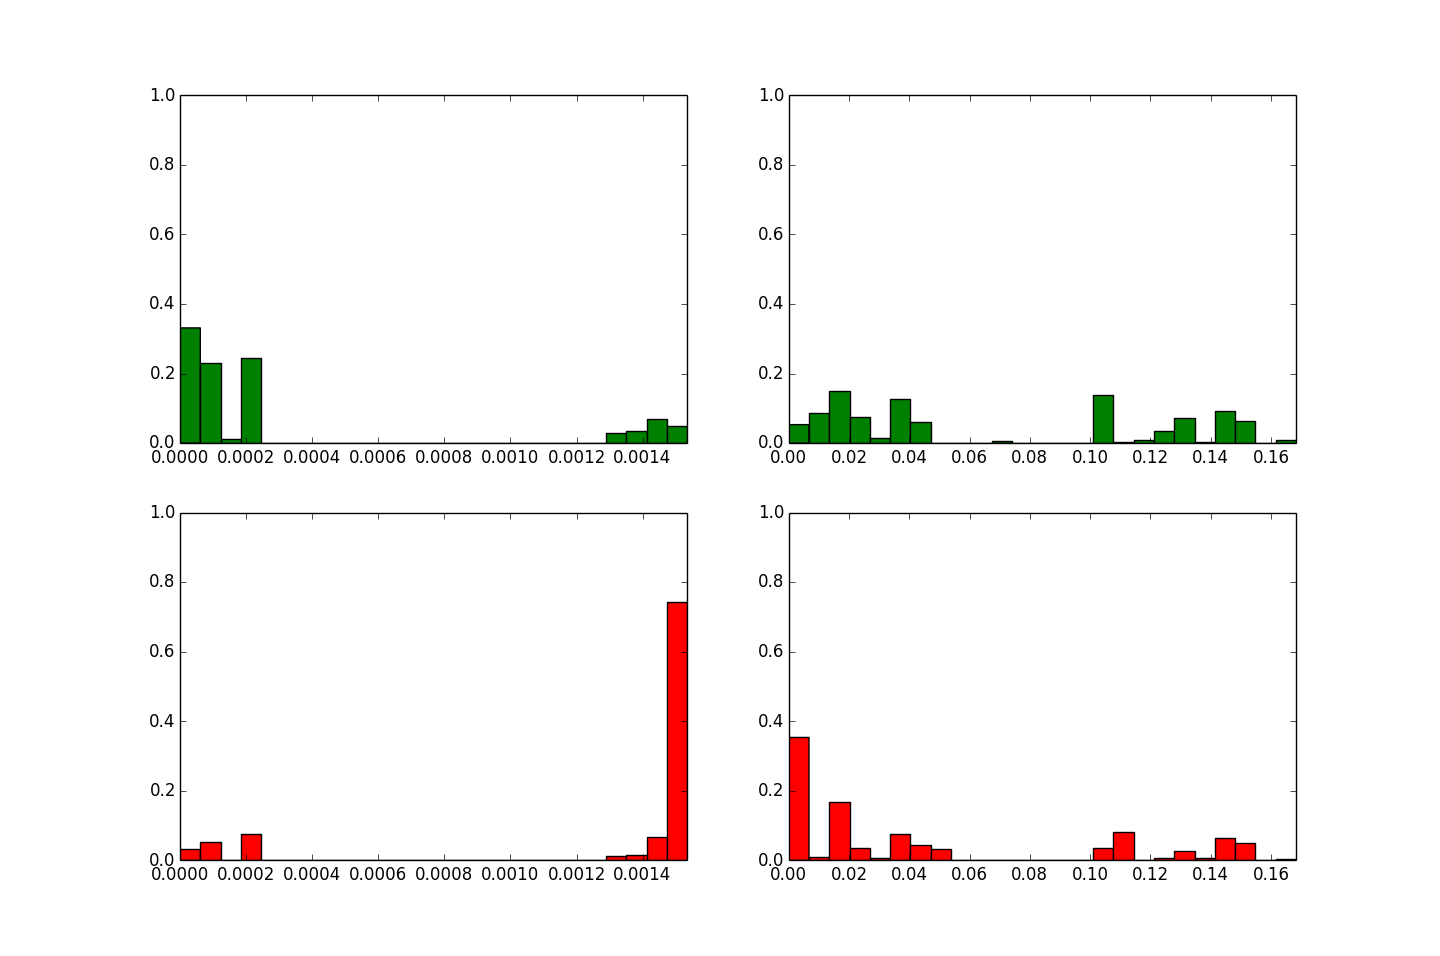
\includegraphics[width =\textwidth]{images/probabilities}
\caption{The distribution in percentages of correct (green) and incorrect (red) document links. Left hand side shows the tag probabilities and the right hand side the link probabilities.}
\label{distribution}
\end{figure}

\subsection{Threshold performance}
The performance of the automated threshold was measured for all vectorizers using the cosine distance metric. Table xx shows the precision and recall for each of the vectorizers, including an unraveling for each type of document. A comparison between this table and table xx, which is measured with the k-link metric, shows that overall, performance does not decrease drastically when using the automated threshold. Setting the correct threshold is always a trade-off between precision and recall. 

